% !TEX program = xelatex

% Základní balíčky
\documentclass[10pt,a4paper]{article}
\usepackage[utf8]{inputenc}
\usepackage[T1]{fontenc}
\usepackage{graphicx}
\usepackage{wrapfig}
\usepackage{nonfloat}
\usepackage{amsmath}
\usepackage{hyperref}
\usepackage{gensymb}
\usepackage[top = 1cm, bottom = 1cm, left = 1cm, right = 1cm]{geometry}

% Language-related
\usepackage[czech]{babel}
\usepackage{csquotes}
\usepackage{polyglossia}
\setmainlanguage{czech}
\setotherlanguage{greek}

% Bibtex je oficiálně mrtka
% \usepackage[backend=bibtex,style=verbose-trad2]{biblatex}
% \usepackage{etoolbox}
% \patchcmd{\thebibliography}{\section*{\refname}}{}{}{}
% \bibliography{protokol}

% Pro titulní stránku
\usepackage{titlesec}
\usepackage{setspace}
\usepackage{framed}
\usepackage{array}

% Vlastní balíčky
\usepackage{gnuplottex}
\usepackage{epstopdf}
\usepackage{csvsimple}
\usepackage{units}
\usepackage{subfig}
\usepackage{pdfpages}

\usepackage{soul}

\usepackage{calc}
\newcommand*{\mask}[2]{\mathord{\makebox[\widthof{\(#1\)}]{\(#2\)}}}




\renewcommand{\U}[1]{\ensuremath{\,\mathrm{#1}}}
\newcommand{\°}{\degree}

\newcommand{\titjmeno}{Michal Grňo}
\newcommand{\titobor}{FOF}


\newcommand{\titcislo}{A6}
\newcommand{\titnazev}{Simulace průchodu částic hadronovým kalorimetrem}
\newcommand{\titmereni}{11. 11. 2020}
\newcommand{\titodevzdani}{18. 11. 2020}


\renewcommand{\t}[1]{\mathrm{#1}}

\begin{document}


\thispagestyle{empty}
\newgeometry{top = 2.5cm, bottom = 0cm, left = 2.5cm, right = 3cm}

{%T tomto je uzavřena celá titulka
%Tloušťka rámečku
\setlength{\fboxrule}{1.5pt}

\noindent
\framebox{
\begin{minipage}{\textwidth}
\setlength{\parindent}{17.62482 pt}
\phantom{d}

\begin{minipage}{0.6\textwidth}
{
\Large Kabinet výuky obecné fyziky, UK MFF\\
}
\vspace*{0.2cm}

{
\bfseries
\huge Fyzikální praktikum %ČÍSLO
}
\end{minipage}
\begin{minipage}{0.4\textwidth}
\begin{center}
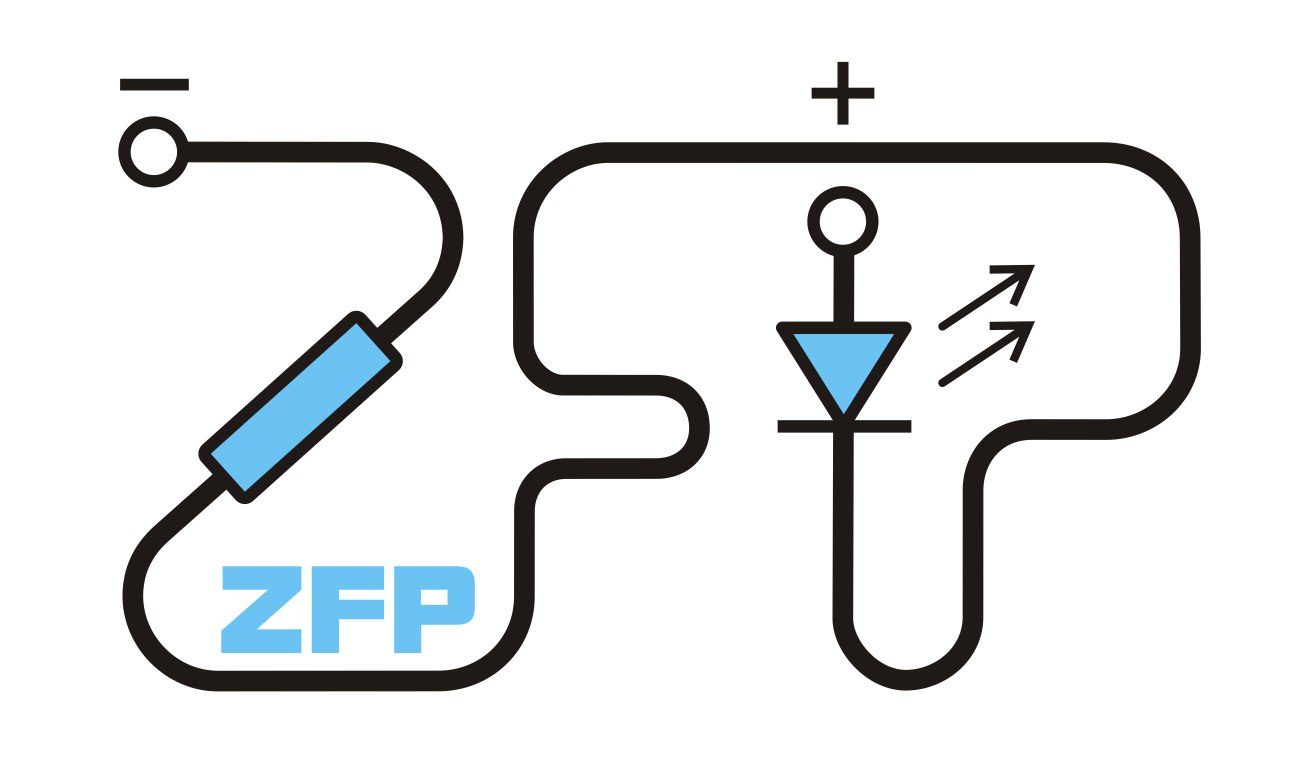
\includegraphics[width=4.5cm]{ZFP.jpg}
\end{center}
\end{minipage}\\\\

%\vspace*{0.5cm}

{
\setstretch{1.5}
\Large
\noindent
Úloha č. \titcislo

\noindent
Název úlohy: \titnazev

\noindent
Jméno: \titjmeno
\hspace*{\fill}
Obor: \titobor

\noindent
Datum měření: \titmereni
\hspace*{\fill}
Datum odevzdání: \titodevzdani

\phantom{d}
}
\end{minipage}
}
%Konec horního rámečku

{
\phantom{d}

\Large
Připomínky opravujícího:\\
\vspace*{6.75cm}
}

\newcommand{\linka}{\noalign{\hrule height 1pt}}
\newcommand{\linkadva}{\noalign{\hrule height 1.5pt}}
\setlength\extrarowheight{9.5pt}
\Large
\noindent
\begin{tabular}{!{\vrule width 1.5pt} l !{\vrule width 1pt} c !{\vrule width 1pt} c !{\vrule width 1.5pt}}
\linkadva
   & Možný počet bodů & Udělený počet bodů \\\linkadva
  Práce při měření & 0-3 &  \\\linka
  Teoretická část & 0-2 &  \\\linka
  Výsledky a zpracování měření & 0-9 &  \\\linka
  Diskuse výsledků & 0-4 &  \\\linka
  Závěr & 0-1 &  \\\linka
  Použitá literatura & 0-1 &  \\\linkadva
  \hspace*{\fill} \textbf{Celkem} \hspace*{\fill}& max. 20 &  \\
\linkadva
\end{tabular}
\phantom{d}

Posuzoval: \hspace*{\fill}dne:~~~~~~~~~~~~~~~~~

}%Konec uzavření titulky
\newpage
\newgeometry{top = 2cm, bottom = 2cm, left = 2cm, right = 2cm}
\setcounter{page}{1}
\setmainfont{Linux Libertine O}




\section{Pracovní úkoly}
\begin{enumerate}
    \item Provést interaktivní simulace základních typů částic a zobrazit jednotlivé interakce
    \item Kvantitativně porovnat energetické ztráty v kalorimetru pro různé druhy částic (elektron, mion, pion)
    \item Prostudovat odezvu modelu kalorimetru a jeho energetické rozlišení
    \item \st{Vypracovat protokol včas, a ne v průběhu noci před odevzdáním}
\end{enumerate}

\section{Teoretická část}
Podstatou úlohy je zpracování a interpretace dat ze simulace kalorimetru pro detekci vysokoenergetických částic. V kalorimetru je možné pozorovat interakce elementárních a složených částic.

Jednou z nejčastěji pozorovaných interakcí je brzdné záření elektronů a pozitronů:
\begin{equation}
    \t e^\pm \to \gamma + \t e^\pm
    \label{brzdne-elektron}
\end{equation}
Vysokoenergetické fotony navíc mohou dát vzniknout páru elektron-pozitron:
\begin{equation}
    \gamma \to \t e^- + \t e^+
    \label{kreace-paru}
\end{equation}
Interakce \eqref{brzdne-elektron} a \eqref{kreace-paru} často probíhají dohromady a tak dávají vzniknout tzv. \textit{elektromagnetické spršce}. Největší roli při absorbování elektromagnetické spršky hraje fotoefekt a Comptonův jev.

Všechny nabité částice navíc mohou ionizovat atomy v kalorimetru:
\begin{equation}
    (\t{částice})^\pm + (\t{atom})^0 \to
    (\t{částice})^\pm + (\t{atom})^+ + \t e^-
    \label{ionizace}
\end{equation}
Uvolněné elektrony mají typicky poměrně malou energii a jsou rychle reabsorbovány.

Interakce mionů $\mu^\pm$ se od elektronů liší tím, že vyzařují mnohem méně brzdného záření a jejich nejčastější interakcí je ionizace atomů \eqref{ionizace}. Dostatečně nízkoenergetické miony jsou typicky zastaveny, načež se rozpadnou na elektron a neutrina a jsou absorbovány:
\begin{equation}
    \begin{aligned}
        \mu^- &\to e^- + \overline{\nu}_{\t e} + \nu_\mu \\
        \mu^+ &\to e^+ + \nu_{\t e} + \overline{\nu}_\mu
    \end{aligned}
    \label{rozpad-mu}
\end{equation}
Takové interakce ovšem nepozorujeme, protože neutrina neinteragují a výsledné elektrony už jsou typicky nízkoenergetické a rychle rekombinují. Na to, abychom interakci pozorovali v okamžiku, kdy má ještě mion vysokou energii, je příliš málo častá.

Dále budeme pozorovat piony $\pi^0, \pi^+, \pi^-$. Ty se velmi rychle rozpadají:
\begin{equation}
    \begin{aligned}
        \pi{\mask{^+}{^0}} &\to \gamma + \gamma \\
        \pi{\mask{^+}{^0}} &\to \t e^- + \t e^+ + \gamma \\
        \pi^+ &\to \t e^+ + \nu_{\t e} \\
        \pi^- &\to \t e^- + \overline{\nu}_{\t e}
    \end{aligned}
    \label{rozpad-pi}
\end{equation}
Výsledkem všech rozpadů jsou elektromagnetické spršky – v případě $\pi^0$ je možné za dobrých podmínek rozlišit dvě nebo tři oddělené spršky.

Interakce hadronů jsou výrazně „nepořádnější“ a méně konzistentní. Pro naše účely stačí shrnout jejich interakce nekonkrétním vztahem:
\begin{equation}
    \t p^\pm, \t e^\pm, \t n^0 \to
    \t p^\pm, \t e^\pm, \t n^0, \pi^\pm, \pi^0, \gamma
    \label{hadronova-sprska}
\end{equation}
Produkty \eqref{hadronova-sprska} se souhrnně označují jako \textit{hadronová sprška}.

Nakonec budeme pozorovat krátkověké neutrální kaony $\t K^0_{\t S}$ a nneutrální $\Lambda$-baryony $\Lambda^0$. Obě tyto částice se mohou rozpadnout na pár neutrálních částic, nebo na kladně a záporně nabitou částici:
\begin{equation}
    \begin{aligned}
        \t K^0_{\t S} &\to \pi^+ + \pi^- &
        \t K^0_{\t S} &\to \pi^0 + \pi^0 \\[3pt]
        \Lambda^0 &\to \t p^+ + \pi^- &
        \Lambda^0 &\to \t n^0 + \pi^0
    \end{aligned}
    \label{kaon-lambda}
\end{equation}
V případě kaonu budeme typicky pozorovat dvě nebo čtyři elektromagnetické spršky, u $\Lambda$-baryonu jednu hadronovou a jednu až dvě elektromagnetické spršky.

V detektoru nebudeme schopni detekovat veškerou energii vstupující částice – část energie budou odnášet například neutrina . Pro pevně určenou vstupní částici o proměnné energii $E_0$, platí, že energie $E_{\mathrm d}$ detekovaná ve scintilátoru kalorimetru je přímo úměrná energii částice: $E_0 \propto E_{\mathrm d}$.

Pro rozlišení $\sigma_E$ reálného detektoru platí vztah:
\begin{equation}
    \underbrace{\sqrt{E_0} \, \frac{\sigma_E}{E_{\mathrm d}}}_{\displaystyle r} = a + b \, \sqrt{E_0} \: ,
    \label{eq-rozliseni}
\end{equation}
kde konstanta $a$ se nazývá \textit{„sampling term“}.

\bigskip

\section{Výsledky měření}
Nejprve jsme měřili $\t e^-, \t e^+, \gamma$. Nezávisle na částici a energii jsme vždy pozorovali typickou elektromagnetickou spršku, viz obr. \ref{obr:em-sprska}. Se zvyšující se energií se sprška pouze zvětšovala, ale nepozorovali jsme žádnou kvalitativní změnu.

\phantom{.}
\begin{minipage}{\linewidth}
    \vspace{\baselineskip}
    \centering
    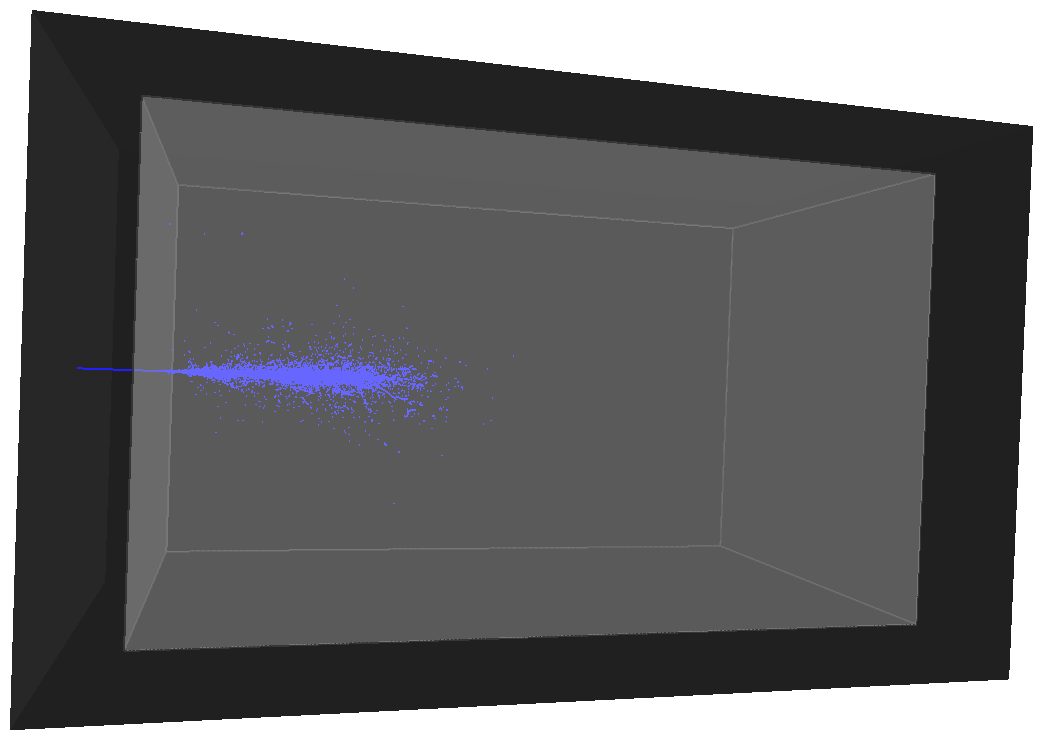
\includegraphics[width=0.6\textwidth]{data/e- 100GeV event0.png}
    \figcaption{Elektromagnetická sprška $\t e^-$ při $100 \U{GeV}$.}
    \label{obr:em-sprska}
    \vspace{\baselineskip}
\end{minipage}

Dále jsme měřili $\mu^\pm$. Pro nízké energie byl mion pouze zpomalen a absorbován (obr. \ref{obr:mu-abs}), při vyšších energiích už proletěl celým kalorimetrem (obr. \ref{obr:mu-prulet}). Při ještě vyšších energiích bylo možné pozorovat ionizaci atomů a při energiích vyšších než $50 \U{GeV}$ začalo být pozorovatelné i brzdné záření (obr. \ref{obr:mu-ioniz}). Kladný i záporný mion produkovaly kvalitativně stejné výsledky.

\phantom{.}
\begin{minipage}{\linewidth}
    \vspace{\baselineskip}
    \centering
    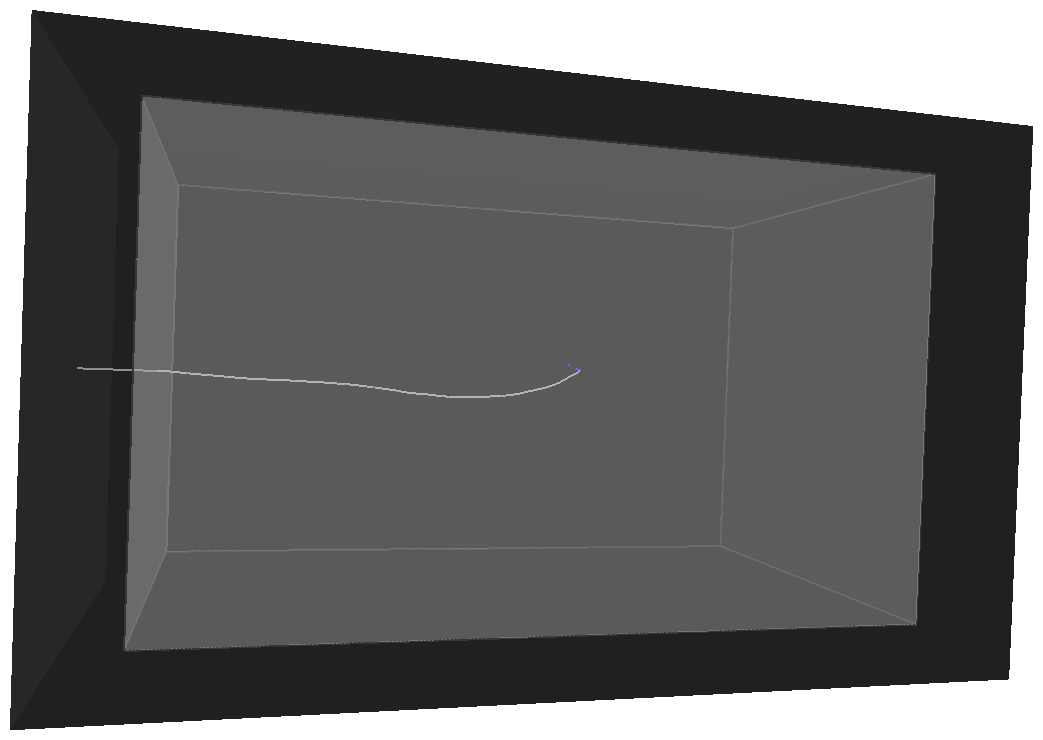
\includegraphics[width=0.6\textwidth]{data/mu+ 1GeV event1.png}
    \figcaption{Absorbce $\mu^+$ při $1 \U{GeV}$.}
    \label{obr:mu-abs}
\end{minipage}

\phantom{.}
\begin{minipage}{\linewidth}
    \vspace{\baselineskip}
    \centering
    \vspace{\baselineskip}
    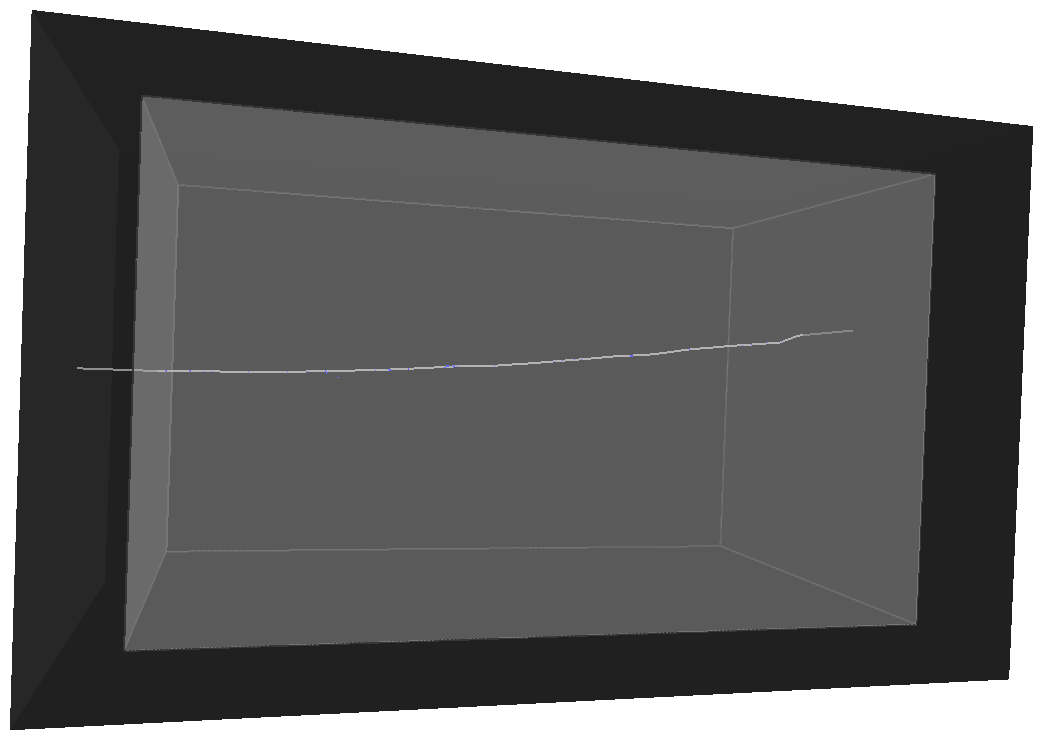
\includegraphics[width=0.6\textwidth]{data/mu- 1.7GeV event6.png}
    \figcaption{Průlet $\mu^-$ při $1.7 \U{GeV}$.}
    \label{obr:mu-prulet}
\end{minipage}

\phantom{.}
\begin{minipage}{\linewidth}
    \vspace{\baselineskip}
    \centering
    \vspace{\baselineskip}
    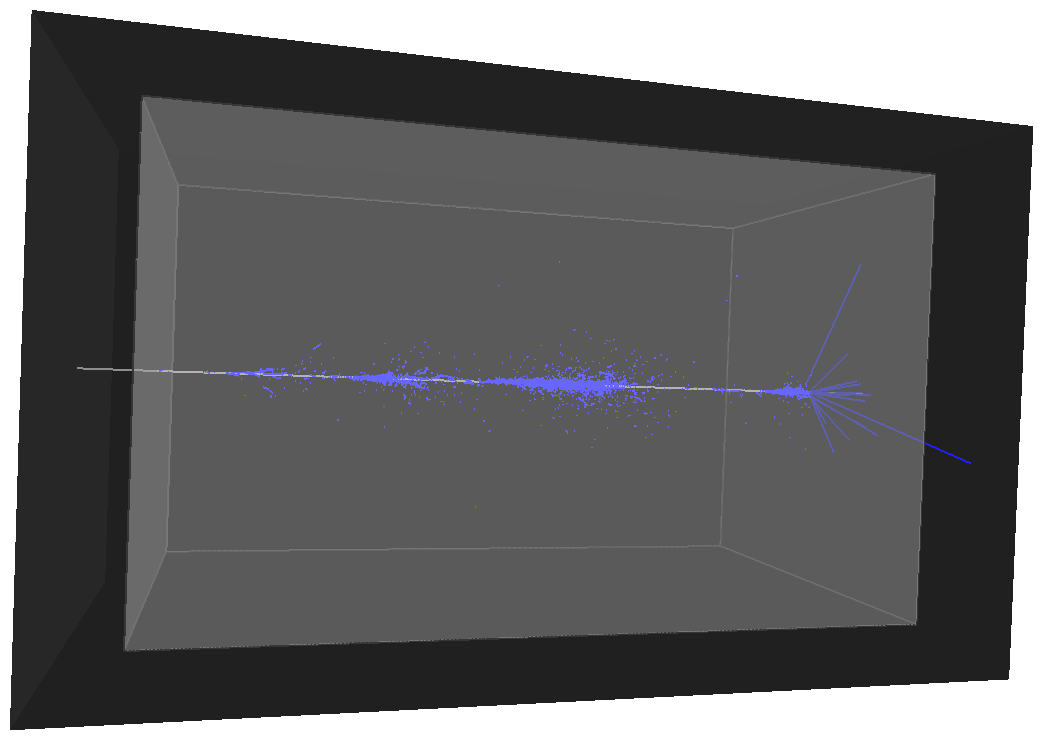
\includegraphics[width=0.6\textwidth]{data/mu- 10000GeV event2.png}
    \figcaption{V levé části ionizace, dále vpravo brzdné záření $\mu^-$ při $10 \U{TeV}$.}
    \label{obr:mu-ioniz}
    \bigskip
\end{minipage}

Následně jsme pozorovali interakce hadronů. O tom, že byly spršky méně konzistentní se můžete přesvědčit z obr.~\ref{obr:protony}.

\begin{wrapfigure}{H}{\linewidth}
    \centering
    \vspace{\baselineskip}
    \subfloat{{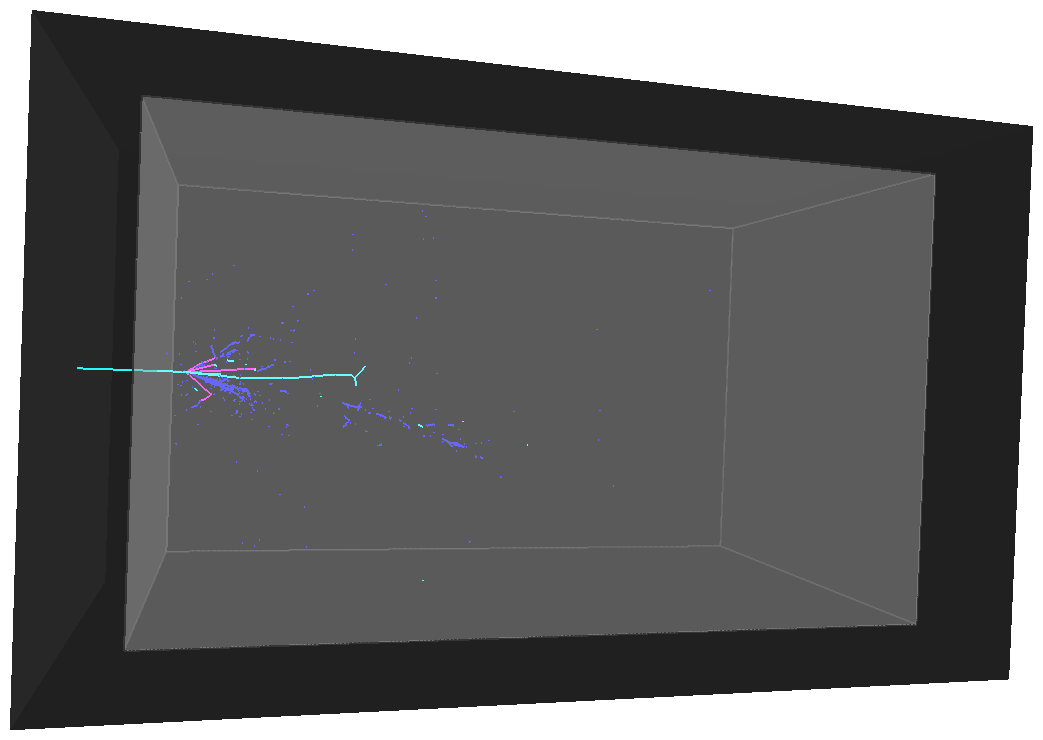
\includegraphics[width=5cm]{data/proton 10GeV event0.png} }}%
    \qquad
    \subfloat{{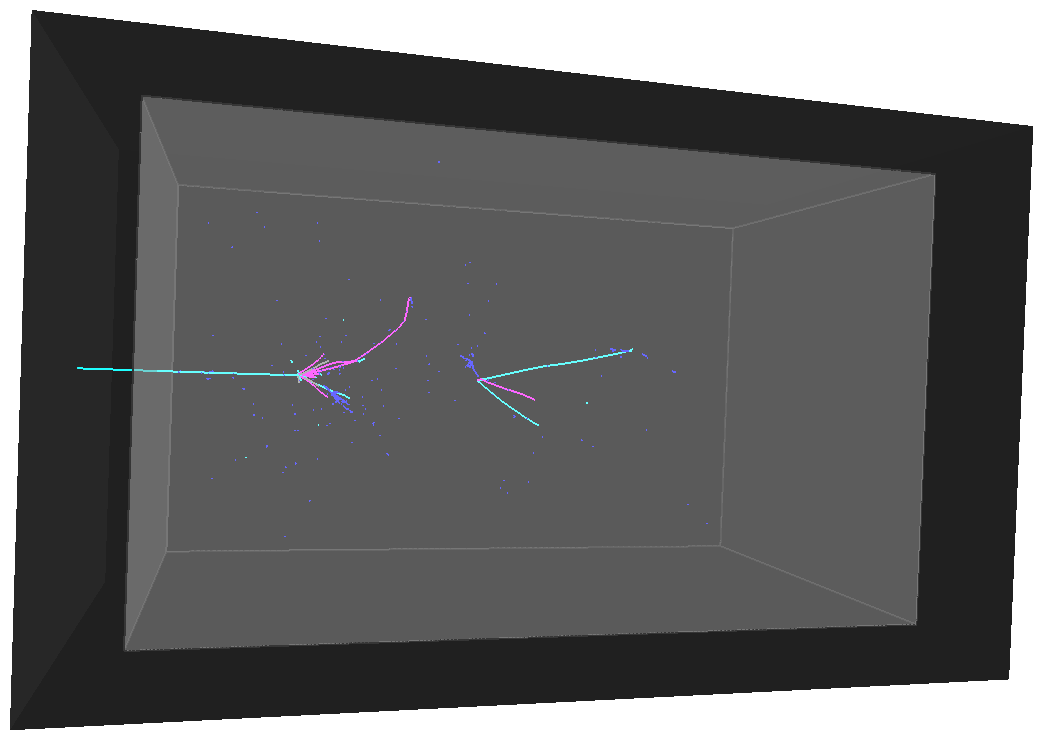
\includegraphics[width=5cm]{data/proton 10GeV event2.png} }}%
    \qquad
    \subfloat{{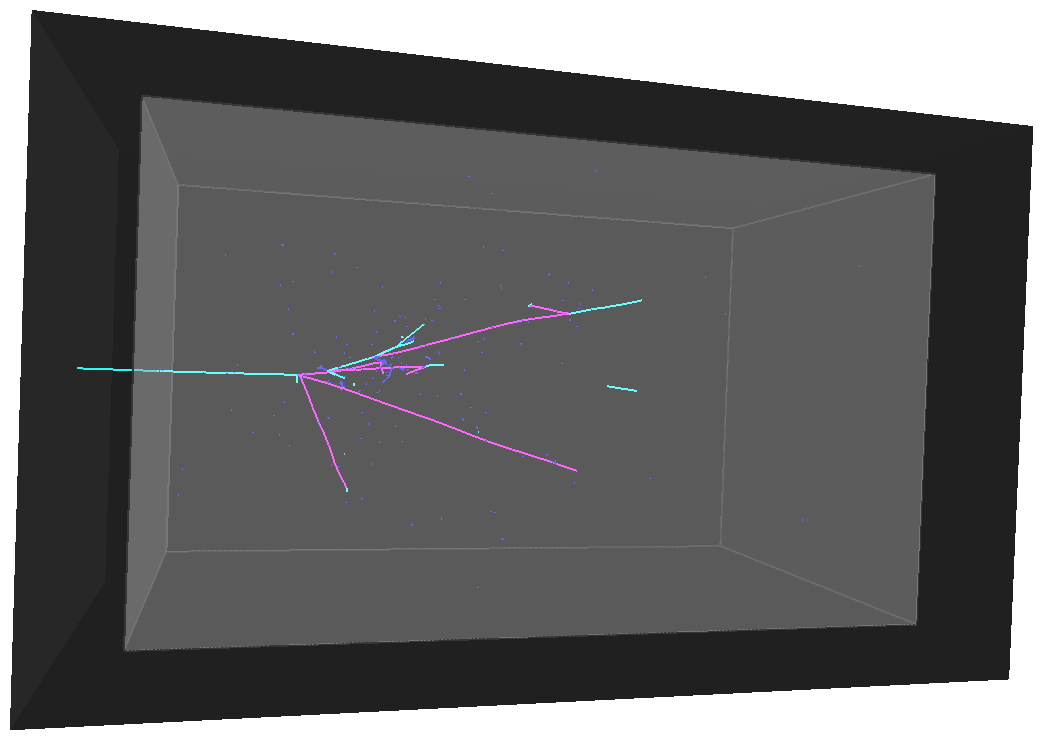
\includegraphics[width=5cm]{data/proton 10GeV event3.png} }}%
    \figcaption{Tři různé interakce $\t p^+$ při $10 \U{GeV}$.}
    \label{obr:protony}
    \vspace{-7cm}
\end{wrapfigure}

\phantom{.}

\pagebreak

\phantom{.}
\begin{minipage}{\linewidth}
    \vspace{\baselineskip}
    \centering
    \vspace{\baselineskip}
    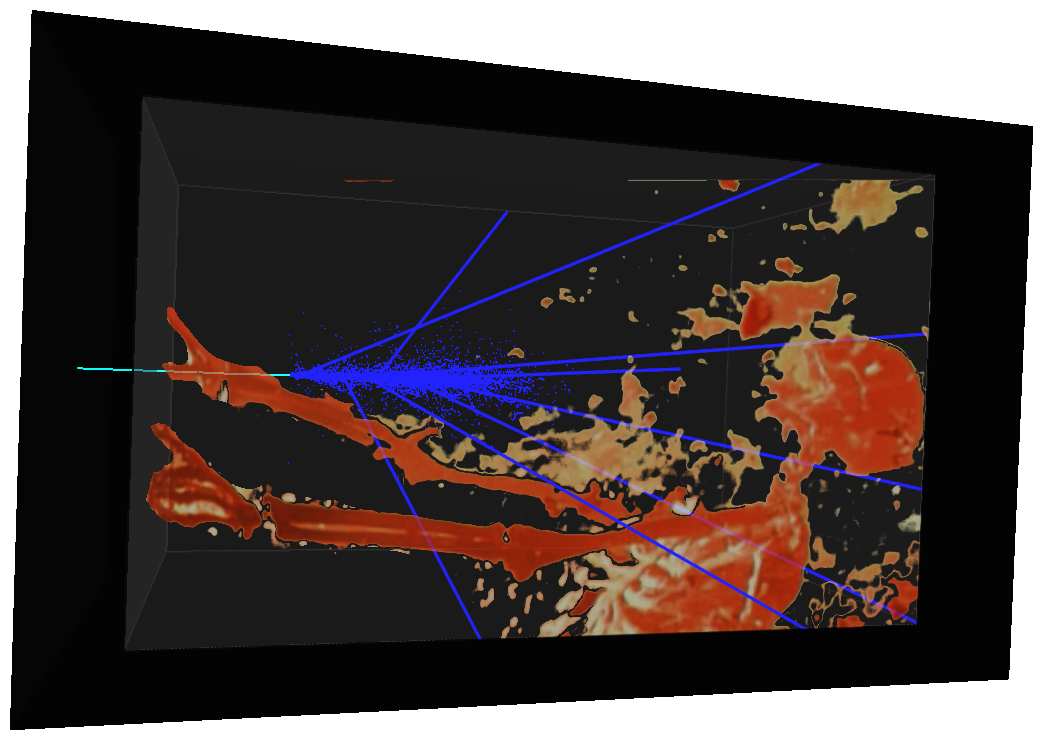
\includegraphics[width=0.6\textwidth]{data/proton decay event0.png}
    \figcaption{Umělecké ztvárnění rozpadu protonu $\t p^+ \to \pi^0 + \t e^+$. Nebylo pozorováno.}
    \label{obr:pi-dva}
    \bigskip
\end{minipage}

Poté jsme měřili $\pi^0$. Jednotlivé elmag. spršky byly rozlišitelné do energií cca $10 \U{GeV}$, poté začaly splývat dohromady a byly těžko rozlišitelné. Případ, kdy by se pion rozpadl na tři částice podle \eqref{rozpad-pi} se nepodařilo identifikovat.

\phantom{.}
\begin{minipage}{\linewidth}
    \vspace{\baselineskip}
    \centering
    \vspace{\baselineskip}
    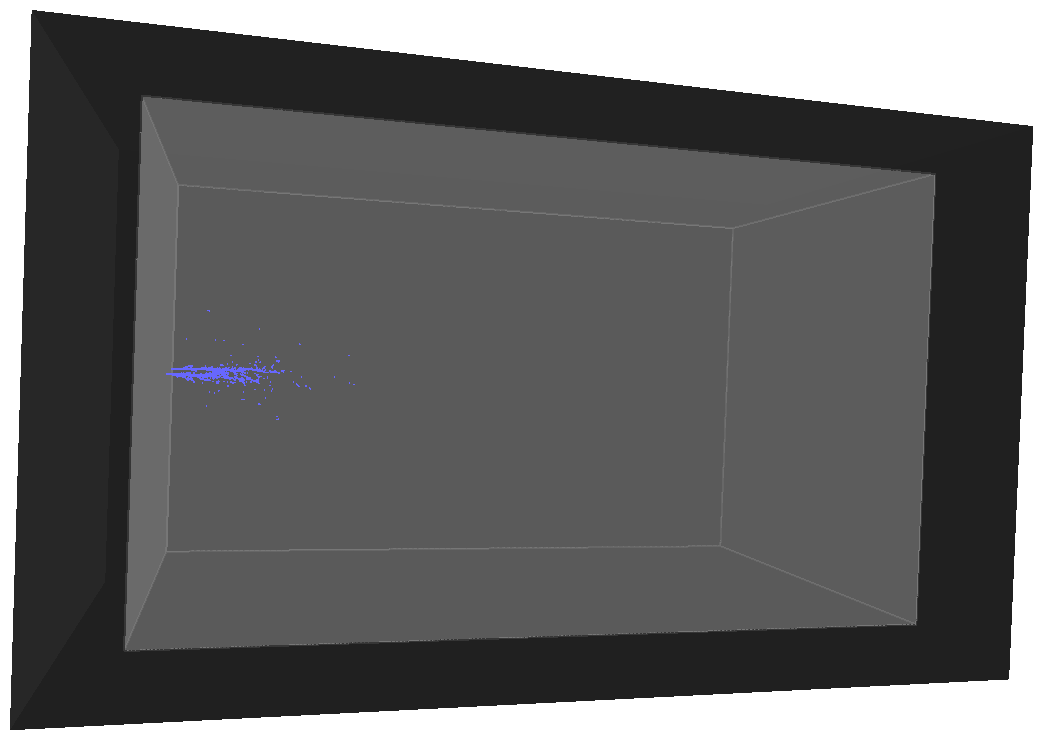
\includegraphics[width=0.6\textwidth]{data/pi0 4GeV event8.png}
    \figcaption{Rozpad $\pi^0$ na dva fotony při $4 \U{GeV}$.}
    \label{obr:pi-dva}
\end{minipage}

Nakonec jsme měřili $\t K^0_{\t S}$, který podle \eqref{kaon-lambda} může mít hadronovou i elektromagnetickou spršku. Obě byly pozorovány (obrázky \ref{obr:kaon-nabite} a \ref{obr:kaon-neutraln}).

\phantom{.}
\begin{minipage}{\linewidth}
    \vspace{\baselineskip}
    \centering
    \vspace{\baselineskip}
    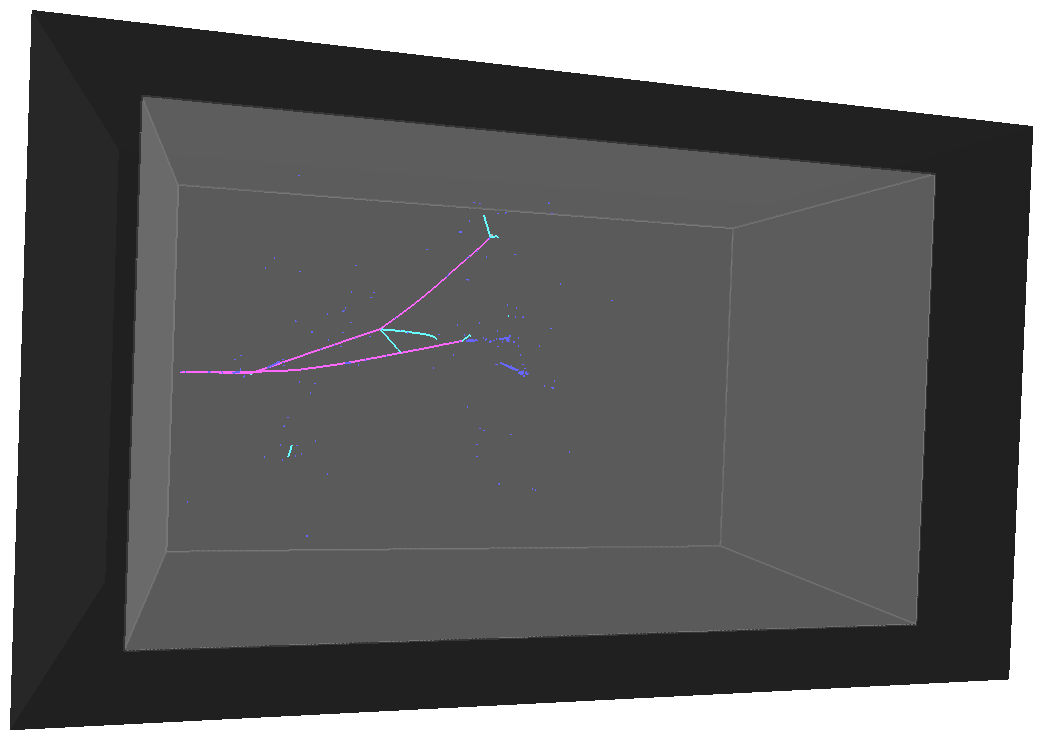
\includegraphics[width=0.6\textwidth]{data/kaon0S 5GeV event3.png}
    \figcaption{Rozpad $\t K^0_{\t S}$ na $\pi^+ + \pi^-$ při $5 \U{GeV}$.}
    \label{obr:kaon-nabite}
\end{minipage}

\phantom{.}
\begin{minipage}{\linewidth}
    \vspace{\baselineskip}
    \centering
    \vspace{\baselineskip}
    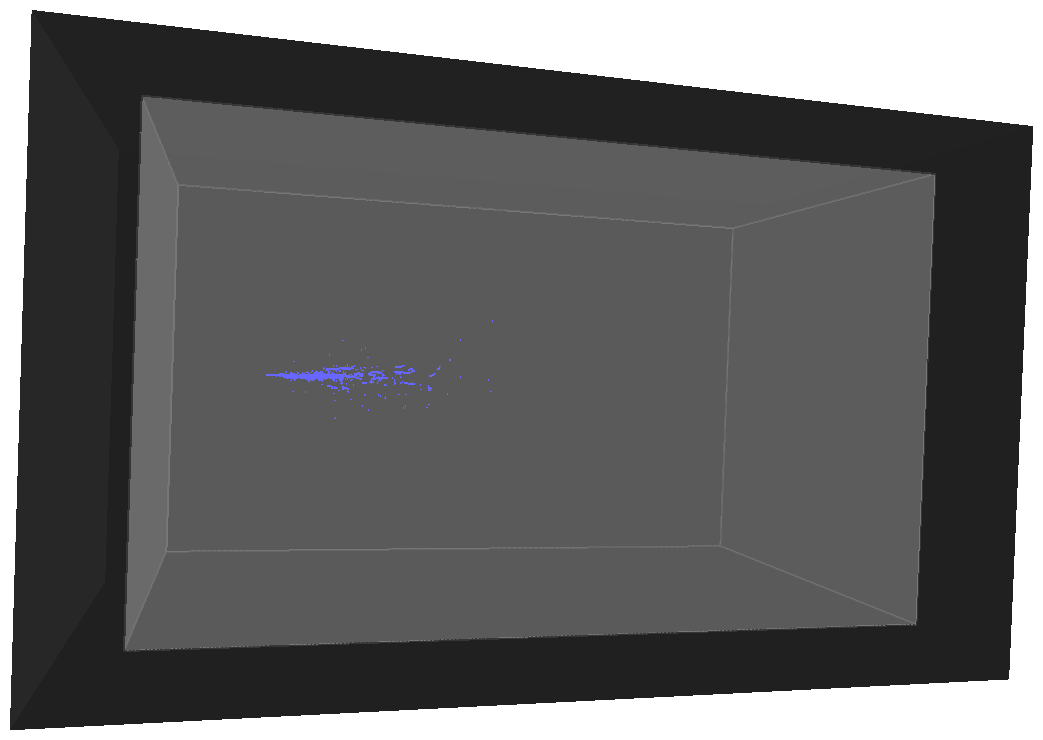
\includegraphics[width=0.6\textwidth]{data/kaon0S 5GeV event4.png}
    \figcaption{Rozpad $\t K^0_{\t S}$ na $2\,\pi^0$ při $5 \U{GeV}$.}
    \label{obr:kaon-neutraln}
    \bigskip
\end{minipage}

Na následujících třech stránkách jsou grafy energetických ztrát částic $\t e^- \!,\, \mu^- \!,\, \pi^+$ (v tomto pořadí) při energii $E_0 = 14 \U{GeV}$.

První ze stránek ukazuje kvantitativní data pro elektron. Součet energií předaných v železné části a ve scintilátoru je $13.54 + 0.42 = 13.99$ (v $\U{GeV}$), drtivá většina produktů interakcí tedy byla absorbována v kalorimetru. Energie předaná ve scintilátoru odpovídá normální distribuci, její rozptyl je cca. $5 \,\%$ střední hodnoty. Bokem kalorimetru unikalo méně než $0.1 \,\%$ celkové energie.

Druhá ze stránek s grafy obsahuje data pro mion. Součet energií předaných v železné části a ve scintilátoru je $11.24 + 0.48 = 11.72$ (v $\U{GeV}$), tedy pouhých $84 \,\%$ vstupní energie. Z grafů energie v závislosti na vzdálenosti vidíme, že skutečně nějaká část mionů unikla. Jedná se ovšem o relativně malý počet mionů, než aby to stačilo k vysvětlení, proč nedetekujeme $16 \,\%$ energie – ve skutečnosti totiž většina nedetekované odchází ve formě mionových a elektronových (anti)neutrin. Energie předaná ve scintilátoru odpovídá normální distribuci, její rozptyl je cca. $10 \, \%$ střední hodnoty. Bokem kalorimetru unikalo cca. $0.13 \,\%$ celkové energie.

Třetí a poslední stránka obsahuje grafy kladného pionu. Tentokrát statistické rozložení předané energie není normální, ale Landauovo. Ze středních hodnot předané energie vidíme, že částice vzniklé interakcemi pionu v kalorimetru typicky zanechají pouze $2.1 \U{GeV}$, tj. $15 \,\%$ vstupní energie. Z grafu energie v závislosti na vzdálenosti je zřejmé, že drtivá většina interagujících částic není v kalorimetru zachycena. Bokem kalorimetru unikalo zanedbatelné množství celkové energie.

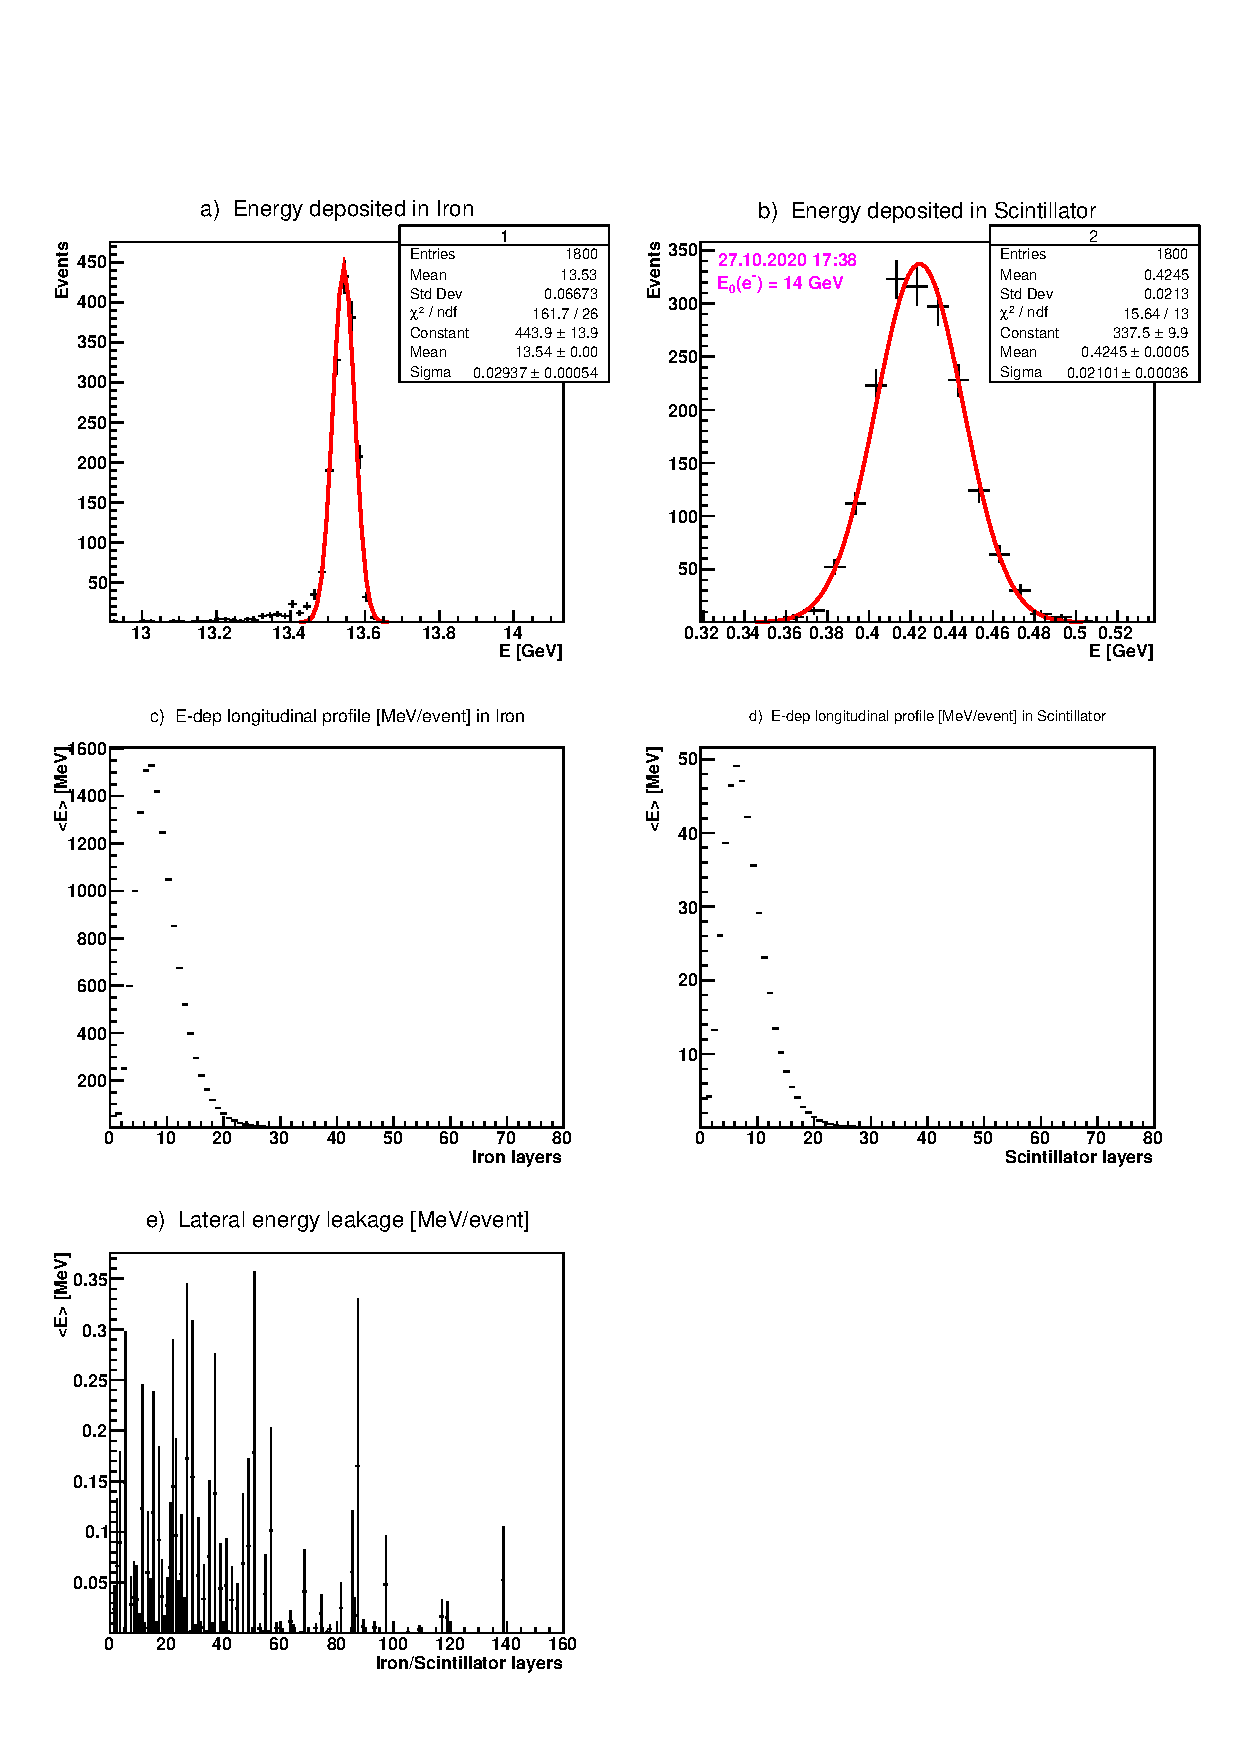
\includepdf[pages=-]{data/14GeV.pdf}

Nakonec jsme detailně zkoumali závislost vstupní energie $E_0$ (v rozpětí $15$ až $55 \U{GeV}$) a energie $E_{\mathrm d}$ předané ve scintilátoru, konkrétně pro vstupní částici $\pi^-$. Chtěli jsme jednak ověřit platnost lineárního vztahu $E_0 \propto E_{\mathrm d}$, ale také určit \textit{samplovací člen} detektoru podle \eqref{eq-rozliseni}. Získaná data byla:

\phantom{.}
\begin{minipage}{\linewidth}
    \vspace{\baselineskip}
    \centering
    \begin{tabular}{ r|rl|rl }
        $E_0 \; [\U{Gev}]$ &
        \multicolumn{2}{c|}{$E_{\mathrm d} \; [\U{Mev}]$} &
        \multicolumn{2}{c}{$r \; [\U{GeV^{\frac{1}{2}}}]$}
        \\\hline
        15.00 &	0.52 &	$\pm$ 0.06 &	45.76 &	$\pm$ 1.47 \\
        25.00 &	0.86 &	$\pm$ 0.11 &	62.93 &	$\pm$ 2.02 \\
        35.00 &	1.18 &	$\pm$ 0.14 &	69.52 &	$\pm$ 2.23 \\
        45.00 &	1.52 &	$\pm$ 0.14 &	60.45 &	$\pm$ 1.93 \\
        55.00 &	1.86 &	$\pm$ 0.16 &	65.13 &	$\pm$ 2.08
    \end{tabular}
    \medskip
    \tabcaption{Závislost celkové a předané energie pro $\pi^-$. Každý řádek je statistickým souborem 500ti událostí.}
    \label{}
    \vspace{\baselineskip}
\end{minipage}

Nejprve jsme sestavili graf $E_{\mathrm d}(E_0)$, viz obr. \ref{graf-energie}. Tím jsme ověřili lineární závislost:
\begin{equation*}
    E_{\mathrm d} = (3.40 \pm 0.02) \cdot 10^{-5} \; E_0
\end{equation*}

Následně jsme provedli afinní fit závislosti $r(\sqrt{E_0})$, viz obr. \ref{graf-rozliseni}, tím jsme získali hodnotu samplovacího členu:
\begin{equation*}
    a = (0.115 \pm 0.052) \U{GeV^{\frac{1}{2}}}
\end{equation*}

\vspace{3\baselineskip}

\phantom{.}
\begin{minipage}{\linewidth}
    \vspace{\baselineskip}
    \centering
    \def\gptboxheight{15cm}
    \begin{gnuplot}[terminal=epslatex,terminaloptions={color size 15cm, 10cm}]
        f(x) = a * x
        fit f(x) 'data/scan.dat' using 1:2:3 yerror via a

        set xrange [10:60]
        set yrange [0.2:2.4]
        set xlabel "$E_0 \\; [\\U{GeV}]$"
        set ylabel "$E_{\\mathrm d} \\; [\\U{MeV}]$"

        plot 'data/scan.dat' skip 1 using 1:2:3 w yerror t 'data', f(x) t 'lineární fit'
    \end{gnuplot}
    \figcaption{Závislost mezi skutečnou vstupní energií a energií detekovanou ve scintilátoru, proložená přímkou procházející počátkem.}
    \label{graf-energie}
    \vspace{\baselineskip}
\end{minipage}

\phantom{.}
\begin{minipage}{\linewidth}
    \vspace{\baselineskip}
    \centering
    \def\gptboxheight{15cm}
    \begin{gnuplot}[terminal=epslatex,terminaloptions={color size 15cm, 10cm}]
        f(x) = a * x + b
        fit f(x) 'data/scan.dat' using 4:(sqrt($1)):5:($2*0.5/sqrt($1)) xyerror via a,b

        set xlabel "$\\sqrt{E_0} \\; [\\U{GeV^{\\frac{1}{2}}}]$"
        set ylabel "$r \\; [\\U{GeV^{\\frac{1}{2}}}]$"

        plot 'data/scan.dat' skip 1 using 4:(sqrt($1)):5:($2*0.5/sqrt($1)) w xyerror t 'data', f(x) t 'afinní fit'
    \end{gnuplot}
    \figcaption{Afinní fit podle vztahu \eqref{eq-rozliseni}.}
    \label{graf-rozliseni}
    \vspace{\baselineskip}
\end{minipage}

\section{Diskuse}
Protože byla data vygenerována simulací, nebyl příliš velký prostor pro nepříjemná překvapení. Přesto by autor chtěl vyjádřit svou rozmrzelost nad faktem, že se nepodařilo naměřit rozpad protonu $\t p^0 \to \pi^0 + \t e^+$, což by dle jeho mínění byla vzrušující událost pro budoucí fyziku a příjemné zpestření středečního dopoledne.

Výsledný \textit{sampling term} je zatížený velkou chybou (asi  $50 \,\%$). Pro lepší kvalitativní posouzení platnosti vztahu \eqref{eq-rozliseni} by tedy bylo vhodné porovnat výsledky i s jinými vstupními částicemi než jen $\pi^-$.

\section{Závěr}
Podařilo se kvalitativně popsat interakce částic $\gamma$, ${\mathrm e}^\pm$, $\mu^\pm$, ${\mathrm p}^+$, $\pi^0$ a ${\mathrm K}_{\mathrm S}^0$ a Kvantitativně prozkoumat předání energie u částic $\t e^- \!,\, \mu^- \!,\, \pi^+$ při $14 \U{GeV}$.

Podařilo se ověřit lineární závislost $E_{\mathrm d} \propto E_0$ a určit \textit{sampling term}, který vyšel:
\begin{equation*}
    a = (0.115 \pm 0.052) \U{GeV^{\frac{1}{2}}}
\end{equation*}


\section{Literatura}
[1] Praktikum částicové a jaderné fyziky. Simulace průchodu vysokoenergetických částic kalorimetrem. Dostupné z: \url{https://physics.mff.cuni.cz/vyuka/zfp/_media/zadani/texty/txt_406.pdf}. 30. září 2014

\vspace{12\baselineskip}

\centering
10 stránek? To jako fakt?!

\end{document}
